% codigoFuenteLibroR2
% Copyright (C) 2020  J.M. Perez Zerpa, et. al.
%
% This program is free software: you can redistribute it and/or modify
% it under the terms of the GNU General Public License as published by
% the Free Software Foundation version 3 of the License.
%
% This program is distributed in the hope that it will be useful,
% but WITHOUT ANY WARRANTY; without even the implied warranty of
% MERCHANTABILITY or FITNESS FOR A PARTICULAR PURPOSE. See the
% GNU General Public License for more details.
%
% You should have received a copy of the GNU General Public License
% along with this program.  If not, see <http://www.gnu.org/licenses/>.

\chapter[Métodos energéticos aplicados a reticulados]{Métodos energéticos aplicados a reticulados}

En esta unidad temática se presentan los conceptos básicos necesarios para abordar el Método de los Desplazamientos (MD) y el Método de las Fuerzas (MF), en ambos casos, aplicados al análisis de estructuras reticuladas. %
%
Se comienza presentando los conceptos de indeterminación cinemática e indeterminación estática  para reticulados planos. %
%
Luego se presenta brevemente el Método de los desplazamientos y finalmente, para realizar el desarrollo del Método de las Fuerzas, se toma como referencias principal \citep{Reddy2002b}.


\section{Grados de indeterminación}

Existen diversos métodos disponibles para el análisis de una estructura, por lo tanto, es útil identificar qué tipo de métodos son los más adecuados \textit{antes} de iniciar el análisis estructural. %
%
En esta sección se presentan propiedades geométricas que pueden ser calculadas \textit{antes} del análisis, para, de esta forma, tomar una mejor decisión sobre el método a utilizar.

Los grados de indeterminación estática y cinemática son valores dados por la geometría y los vínculos existentes entre componentes de la estructura. %
%
Estos valores numéricos permiten estimar la complejidad de la resolución usando dos métodos analíticos presentados el curso: el \textit{Método de las Fuerzas} y el \textit{Método de los Desplazamientos}. %
%


\subsection{Grado de indeterminación cinemática}

El grado de indeterminación cinemática permite establecer la cantidad de incógnitas cinemáticas que se deben determinar para conocer el desplazamiento de todos los puntos de la estructura.
%
Una posible expresión matemática de este parámetro es:
%
\begin{equation}
	gk = g_l \, n_N - c_a,
\end{equation}
%
donde $g_l$ es el número de grados de libertad por nodo, $n_N$ es el número de nodos de la estructura y $c_a$ el número de grados de libertad conocidos por las condiciones de apoyo o vínculo a tierra. %
%
En estructuras articuladas planas $g_l$ es 2, en estructuras aporticadas planas $g_l=3$ y en aporticadas tridimensionales $g_l=6$.

El grado de indeterminación cinemática permite conocer el número de incógnitas de los sistemas de ecuaciones planteados al usar el Método de los Desplazamientos o sus variantes computacionales como el Método de los Elementos Finitos.

En el caso de la estructura mostrada en la Figura~\ref{fig:retic_gh}, se puede ver que $gk=2\times 4 - 4=4$.


\subsection{Grado de indeterminación estática}

% -------------------------
El grado de indeterminación estática (también llamado \textit{grado de hiperestaticidad}) es un valor numérico definido por la diferencia entre: el número de incógnitas de fuerza y el número de ecuaciones de equilibrio. %
%

\subsubsection{Grado de hiperestaticidad de reticulados}

En el caso particular de reticulados planos es posible obtener una forma simplificada de cálculo. %
% 
El estado tensional de las estructuras formadas por barras articuladas queda definido a partir de los valores de tensiones axiales o las directas de las barras (una incógnita por barra), y por las reacciones en cada uno de los vínculos a tierra. %
%
Cada barra introduce una directa como incógnita, mientras que cada componente de fuerzas de reacción también debe ser considerado (una incógnita por cada dirección).

Para las ecuaciones de equilibrio, en problemas planos, se cuenta con dos ecuaciones de equilibrio por cada nodo (cuerpo libre), por lo que el grado de hiperestaticidad puede ser escrito como
%
\begin{equation}
	\boxed{
	gh = n_R + n_{B} - 2 \times n_{N}
}
\end{equation}
%
donde $n_R$ es el número de reacciones a determinar, $n_B$ es el número de barras de la estructura y $n_N$ es el número de nodos.

En la estructura de la Figura~\ref{fig:retic_gh} se puede ver un reticulado formado por 6 barras con dos apoyos fijos. Se tienen $n_B=6$ solicitaciones por tener 6 barras, y $n_R=4$ por tener 2 reacciones en cada nodo apoyado fijo. %

\begin{figure}[htb]
	\centering
	\def\svgwidth{0.5\textwidth}
	\input{figs/UT1/retic_gh.pdf_tex}
	\caption{Ejemplo reticulado plano hiperestático.}
	\label{fig:retic_gh}
\end{figure}

Por otra parte, si se considera cada nodo de la estructura como un componente aislado se pueden plantear dos ecuaciones de equilibrio de fuerzas a cada componente, por lo tanto se tiene:
%
\begin{equation}
	gh = 4 + 6 - 2 \times 4 = 2.
\end{equation}

Tener una estructura con grado de hiperestacidad 2, es equivalente a decir que si se aplican las ecuaciones de equilibrio únicamente, tendríamos un sistema \textbf{compatible indeterminado}. El subespacio de soluciones del sistema será de dimensión 2.




\subsubsection{Clasificación de estructuras según grado de hiperestaticidad} %

Las estructuras pueden ser clasificadas según su grado de hiperestaticidad de la siguiente manera:

\begin{itemize}
	\item \textit{estáticamente determinada} (o isostática): es aquella estructura cuyo estado tensional puede ser determinado usando únicamente ecuaciones de equilibrio, por lo tanto:
	$$
	gh = 0
	$$
	
	\item \textit{hiperestáticas}: es aquella estructura para la cual no es posible determinar el estado tensional usando únicamente equilibrio, es decir:
	$$
	gh > 0.
	$$
	En este caso deben ser utilizadas oras ecuaciones como por ejemplo compatibilidad de desplazamientos. %
	
	\item \textit{hipoestáticas} (o mecanismos): este último caso corresponde a estructuras en las cuales se tienen más ecuaciones que incógnitas por lo tanto
	$$
	gh <0.
	$$
\end{itemize}




\subsubsection{Grado de hiperestaticidad externa}
%
Si la estructura puede ser considerada como un conjunto (sin mecanismos internos)  es posible definir el concepto de grado de hiperestaticidad externa como:
%
\begin{equation}
	gh_E = n_{R} - 3
\end{equation}
%
donde $n_R$ es nuevamente el número de reacciones. %
%

Finalmente, se puede usar los valores $gh_E$ y $gh$ para formular una condición \textbf{necesaria} que una estructura \textit{isostática} debe cumplir. %
%
Se dice que:
%
$$
\boxed{
	\text{Estructura isostática} \quad \Rightarrow \quad gh_E = 0 \quad \textbf{y} \quad gh = 0.
}%
$$
% -------------------------


%Existen casos de particulares, de estructuras en las cuales aún siendo isostáticas el grado de hiperestaticidad externa es mayor que cero, como por ejemplo la mostrada en la Figura~\ref{fig:hipereje}. %
%%
%Esto se debe a que la estructura está conformada por barras no conectadas entre sí como ocurre en la mostrada en las Figuras \ref{fig:ejemghMed} o \ref{fig:retic_gh}. %
%%
%Esta peculiaridad teórica no será relevante al momento de aplicación práctica del Método de las Fuerzas como se verá en la UT siguiente.





\subsubsection{Grado de hiperestaticidad para estructuras aporticadas}

Al considerar estructuras aporticadas, las ecuaciones deben ser modificadas y la complejidad en el cálculo aumenta. Este tipo de cálculo de $gh$ puede ser necesario si el Ingeniero analista cuenta con el Método de las Fuerzas como una de las opciones a aplicar en su análisis. Los estudiantes interesados en los métodos más generales de cálculo pueden consultar referencias como \citep{CerveraRuiz2002ii}. %
%


%En esta metodología se parte de un EBC, opcionalmente se pueden considerar componentes separadas de la estructura y se aplica una ecuación para el cálculo.
%
%Las \textbf{incógnitas de fuerza} son aquellas necesarias para determinar completamente el \textit{\textbf{estado tensional}} de toda la estructura. En las estructuras consideradas en este texto, estas incógnitas son:
%%
%\begin{itemize}
%	\item $n_S$: solicitaciones a determinar y fuerzas debidas a \textit{vínculos internos} de cada componente,
%	\item $n_R$: reacciones dadas por \textit{vínculos externos}.
%\end{itemize}
%
%
%Por otra parte para calcular el número de ecuaciones con que se cuenta se define:
%%
%\begin{itemize}
%	\item $n_C$: es el número de componentes o partes en la que se separa la estructura para el cálculo,
%	\item $n_E$: el número de ecuaciones de equilibrio para cada parte.
%\end{itemize}
%
%La expresión matemática del grado de indeterminación estática puede ser presentada como:
%%
%\begin{equation} \label{eqn:gradoh}
%	gh = n_R + n_S - n_C \, n_{E}.
%\end{equation}
%
%Como ejemplo se presentan las estructuras de la Figura~\ref{fig:ejemghSimp}, formadas por un único componente y con diferente cantidad de reacciones externas. Dado que no se cortan o liberan vínculos internos de la estructura no hay $n_S$.
%
%\begin{figure}[htb]
%	\centering
%	\def\svgwidth{0.95\textwidth}
%	\input{figs/UT1/ejemplos_basicosGradoHiper.pdf_tex}
%	\caption{Ejemplos simples de cálculo de grado de hiperestaticidad.}
%	\label{fig:ejemghSimp}
%\end{figure}
%
%En la Figura~\ref{fig:ejemghMed}. se muestra un reticulado, donde nuevamente si se desacopla en $n_C=3$ componentes una por barra, se tiene que cada articulación introduce dos vínculos a determinar. Por lo tanto $gh = 2+1+2+2+2-3\times 3 = 0$.
%
%\begin{figure}[htb]
%	\centering
%	\def\svgwidth{0.6\textwidth}
%	\input{figs/UT1/ejemplos_mediosGradoHiper.pdf_tex}
%	\caption{Ejemplo de cálculo de grado de hiperestaticidad en reticulado.}
%	\label{fig:ejemghMed}
%\end{figure}
%
%Este cálculo también puede ser realizado considerando la estructura como una única componente. Más adelante se mostrará una ecuación práctica para el cálculo de $gh$ en reticulados planos.
%
%\paragraph{Analogía con cálculo a partir de grados de libertad} %
%El cálculo presentado es análogo al utilizado en otros cursos, en los cuales se considera el número de grados de libertad total de las estructuras (en el ejemplo $3\times 3$) y se van restando los vínculos que restringen el movimiento entre barras y a tierra ($-2-1-2-2-2$) por lo que se obtiene un valor opuesto al $gh$.
%
%
%
%
%
%
%
%
%\subsubsection{Cálculo general de grado de hiperestaticidad en pórticos/vigas/barras planos}
%
%En el caso de estructuras de pórticos planos, la determinación del estado tensional requiere conocer 3 solicitaciones en todo punto: directa, cortante y momento. %
%%
%A modo de ejemplo se considera la estructura mostrada en la Figura~\ref{fig:gerb}: en la parte superior se muestra el esquema básico con la carga aplicada, mientras que en la parte inferior se muestra una de las formas en que la estructura puede ser separada en componentes. 
%%
%\begin{figure}[htb]
%	\centering
%	%
%	\def\svgwidth{0.7\textwidth}
%	\input{figs/UT1/ejemplo_grado_hiper.pdf_tex}
%	%
%	\caption{Ejemplo de grado de indeterminación estática: estructura con cargas aplicadas (superior) y estructura con componentes separadas y cantidad de reacciones incógnita (inferior).}
%	\label{fig:gerb}
%\end{figure}
%
%La cantidad de solicitaciones a determinar en cada vínculo es indicado con un círculo y el cálculo del grado de hiperestaticidad usando la Ecuación~\eqref{eqn:gradoh} está dado por:
%%
%\begin{equation}
%	n_R = 3+1+1 \quad n_S = 2+2 \quad n_C = 3 \quad n_E = 3 \quad \Rightarrow \quad gh = 0
%\end{equation}
%%
%por lo tanto la estructura es isostática.
%
%El $gh$ es un parámetro útil para estimar la complejidad de la aplicación del Método de las Fuerzas. %
%%
%Dado que en este texto dicho método es desarrollado únicamente para reticulados, el cálculo del $gh$ para pórticos no es abordado de forma extensiva. %
%%
%En la Sección 1.6 de \citep{CerveraRuiz2002ii} se presenta un desarrollo más extenso sobre la determinación del grado de hiperestaticidad así como también se muestran diversos ejemplos.
%
%
%





\section{Método de los Desplazamientos}

El desarrollo presentado en esta sección está enfocado a la versión matricial del MD para elementos de barra de dos nodos sin fuerzas de volumen y de sección transversal uniforme. %
%

Al desarrollar métodos de análisis de estructuras se utilizan hipótesis vinculadas al desplazamiento de los distintos elementos estructurales. %
De forma general se puede decir que los desplazamientos de todos los puntos de una estructura están dados por una suma de funciones de interpolación $\phi_i$ multiplicadas por los desplazamientos de los nodos de referencia de la estructura $u_i$:
%
\begin{equation}
u(P) = \sum_{i=1}^{n_d} u_i \phi_i(P),
\end{equation}
%
donde $P$ representa un punto cualquiera de la estructura y $n_d$ es el número de desplazamientos de referencia de la estructura (o número de incógnitas cinemáticas). %


El vector de todos los desplazamientos de referencia $\bfu \in \bbR^{n_d}$ brinda toda la información necesaria para construir la función de desplazamiento de toda la estructura (con el grado de aproximación brindado por las funciones $\phi$). %
%
Las funciones $\phi$ pueden ser tales que el desplazamiento de cada punto es una combinación lineal de los desplazamientos de los nodos extremos correspondientes.

Como ejemplo se considera el reticulado mostrado en la Figura~\ref{fig:retic_gh} se puede considerar que el desplazamiento de cualquier punto de las barras puede ser interpolado a partir de los desplazamientos de los nodos, por lo que se tendrían $8$ desplazamientos de referencia (dos por nodo).

Por otra parte, en cada nodo donde se definen desplazamientos de referencia $u_i$ se pueden considerar fuerzas externas aplicadas $f_i$.

\subsection{Interpolación lineal de desplazamientos}

En el caso de estructuras de barras articuladas, las funciones de interpolación pueden ser consideradas lineales en el dominio correspondiente a cada barra, siendo los desplazamientos de los nodos articulados los desplazamientos de referencia. %
%
Esto puede ser escrito para cada barra $e$ de la estructura usando las funciones lineales de interpolación:
%
\begin{equation}
\bfu (x^e) = \bfN^e(x^e) \bfu^e,
\end{equation}
%
donde $x^e$ es una coordenada local del elemento, $\bfN^e$ es la matriz de funciones de interpolación de la barra y $\bfu^e$ es el vector columna de los desplazamientos de los nodos de la barra. %
%


Se considera ahora elementos de barra como el mostrado en la Figura~\ref{fig:eleplabar} para los cuales sus movimientos están incluidos en un plano $x-y$. %
%
\begin{figure}[htb]
	\centering
  \def\svgwidth{0.6\textwidth}
  \input{figs/UT2/sistcord.pdf_tex}
	\caption{Esquema de sistemas de coordenadas de elemento de barra en el plano.}
	\label{fig:eleplabar}
\end{figure}

El desplazamiento según el eje de la barra, coincidente con el eje de coordenadas $x$ local, está dado por:
%
\begin{equation}
u_L^e(x^e) = N_1^e(x^e) u_{1,L}^e  + N_2^e(x^e) u_{2,L}^e,
\end{equation}
%
donde las funciones de interpolación están dadas por
%
\begin{equation}
N_1^e(x^e) = \frac{\ell^e - x^e}{\ell^e}
\quad \text{y} \quad N_2^e(x^e) = \frac{x^e}{\ell^e},
\end{equation}
%
siendo $\ell^e$ el largo de la barra $e$.


%
Usando la relación de deformación-desplazamiento y derivando (respecto a la coordenada local) se obtiene la expresión de la deformación en el dominio del elemento:
%
\begin{equation}
\varepsilon^e(x^e) = \frac{\partial u^e_L}{\partial x^e}(x^e) =  B_{1,L}^e(x^e) u_{1,L}^e  + B_{2,L}^e(x^e) u_{2,L}^e
\end{equation}
%
donde 
\begin{equation}
B_{1,L}^e(x^e) = \frac{- 1}{\ell^e}
\quad \text{y} \quad B_{2,L}^e(x^e) = \frac{1}{\ell^e},
\end{equation}
son las derivadas de las funciones de interpolación respecto a la coordenada local. %
%
Se observa que, para esta interpolación, la deformación axial es uniforme en todo el elemento (es decir que no depende de $x^e$) y vale 
%
\begin{equation}
\varepsilon^e  =  \frac{ u_{2,L}^e - u_{1,L}^e } {\ell^e}.
\end{equation}


Esto puede ser escrito en forma matricial como:
%
\begin{equation} \label{eqn:expreps}
\varep^e (\bfu^e_L) = \bfB_L^e \bfu^e_L,
\end{equation}
%
donde,
%
\begin{equation}
\bfB_L^e = \frac{1}{\ell^e} \left[-1, 0, 1, 0\right]
\quad \text{y} \quad
\bfu_L^e = \left[u_{1,L}, v_{1,L}, u_{2,L}, v_{2,L}\right]^T.
\end{equation}

Usando la ecuación constitutiva lineal se obtiene la tensión de cada elemento como:
%
\begin{equation}\label{eqn:barraeccons}
\sigma^e = E^e \varepsilon^e,
\end{equation}
donde $E^e$ es el módulo de Young del elemento o barra $e$ y $\sigma^e$ es la tensión axial, también uniforme en el elemento.


\subsection{Energía potencial total}

Para poder aplicar esta interpolación a los principios energéticos es necesario obtener una expresión de la energía potencial total de la estructura en función de los desplazamientos nodales. %
%
Para esto se sustituyen las expresiones obtenidas en las definiciones de la energía potencial de deformación elástica $\Pi_{int}$ y la energía potencial de las fuerzas externas $\Pi_{ext}$.

La energía potencial de deformación de cada barra está dada únicamente por la componente axial. Usando la expresión general dada por la Ecuación~\eqref{eqn:energbarra} y la forma del tensor de deformación dada por la Ecuación~\eqref{eqn:epsbarras}, se obtiene:
%
\begin{equation}
\Pi_{int}^e (\bfu_L^e) %
%
= \frac{1}{2} \int_{\Omega^e} E^e \left(\varepsilon^e (\bfu_L^e) \right)^2 \dif V ,
%
\end{equation}
%
donde $\Omega^e$ representa el volumen ocupado por la barra $e$. %
%
Sustituyendo la relación de la Ecuación~\eqref{eqn:expreps} y operando se obtiene:
%
\begin{equation}
\Pi_{int}^e(\bfu_L^e) = \frac{1}{2} (\bfu_L^e)^T \bfK_L^e \bfu_L^e ,
\end{equation}
%
donde $\bfK_L^e$ es una matriz dada por:
%
\begin{equation}\label{eqn:defK}
 \bfK_L^e = \int_{0}^{\ell^e} (\bfB_L^e)^T E^e A^e \bfB_L^e \dif x.
\end{equation}
%
La expresión desarrollada es:
%
\begin{equation}
\bfK_L^e = \frac{E^e A^e}{\ell^e} 
\left[
\begin{matrix}
1 & 0 & -1 & 0 \\
0 & 0 & 0 & 0\\
-1 & 0 &  1 & 0\\
0 & 0 & 0 & 0
\end{matrix}
\right].
\end{equation}
%

Para poder resolver problemas con varios elementos de barra, con sus ejes orientados en diferentes direcciones, es necesario trabajar con un sistema de coordenadas global. %
%
Considerando que el sistema de coordenadas local del elemento forma un ángulo $\alpha^e$ como se muestra en la Figura~\ref{fig:eleplabar} (medido antihorario desde el sistema global), la matriz de cambio de base $\bfR^e$ está dada por:
%
\begin{equation}\label{eqn:rotabarra}
\bfR^e = 
\left[
\begin{matrix}
c & -s & 0 & 0 \\
s & c & 0 & 0\\
0 & 0 &  c & -s\\
0 & 0 & s & c
\end{matrix}
\right]
\qquad
\bfu^e = \bfR^e \bfu^e_L
\end{equation}
%
donde $c=\cos(\alpha^e)$ y $s=\sin(\alpha^e)$ y $\bfu^e$ es el vector de desplazamientos del elemento en coordenadas globales. %
%

\cajaactividad{
Demostrar la identidad dada por la Ecuación~\ref{eqn:rotabarra} aplicando la relación de cambio de base vista en cursos de Álgebra Lineal:
$$
\text{coord}_B(\bfu) = 
_B(\bfI)_A
\text{coord}_A(\bfu),
$$
y la definición de matriz asociada de una transformación lineal.
}

Sustituyendo este cambio de coordenadas en la expresión de la energía potencial de deformación se tiene
\begin{equation}
\Pi_{int}^e(\bfu^e) = \frac{1}{2} (\bfu^e)^T \bfK^e \bfu^e,
\end{equation}
%
donde la matriz $\bfK^e$ en coordenadas globales está dada por:
%
\begin{equation}
\bfK^e = \bfR^e \bfK^e_L (\bfR^e)^T
= 
\frac{E^e A^e}{\ell^e}
\left[
\begin{matrix}
c^2 & cs & -c^2 & -cs \\
cs & s^2 & -cs & -s^2\\
-c^2 & -cs &  c^2 & cs\\
-cs & -s^2 & cs & s^2
\end{matrix}
\right].
\end{equation}




La energía potencial de deformación de toda la estructura puede ser calculada sumando las energías de las $n_e$ barras que forman la estructura:
%
\begin{equation}\label{eqn:matU}
  \Pi_{int}(\bfu) = \sum_{e=1}^{n_e} \Pi_{int}^e(\bfu^e) = 
   \sum_{e=1}^{n_e} \frac{1}{2} (\bfu^e)^T \bfK^e \bfu^e 
= \frac{1}{2} \bfu^T \bfK \bfu
\end{equation}
%
donde $\bfK$ es la versión \textit{ensamblada} de las matrices $\bfK$ y $\bfu$ es el vector de todos los deplazamientos nodales de la estructura.



Las fuerzas externas aplicadas son representadas por el vector $\bff_{ext}$ o simplemente $\bff$. %
%
La energía potencial de estas fuerzas es representada por $\Pi_{ext}$ y está dada por:
%
\begin{equation}
 \Pi_{ext}(\bfu) = - \sum_{i=1}^{n_d} u_i f_i = - \bfu^T \bff .
\end{equation}
%

La energía potencial total estará dada por lo tanto, por la suma de ambas energías:
%
\begin{equation}
\boxed{
\Pi(\bfu) = \frac{1}{2} \bfu^T \bfK \bfu - \bfu^T \bff .
}
\end{equation}



\subsection{Desarrollo del método}

Los principios energéticos brevemente descritos en la Unidad Temática 1 pueden ser revisados nuevamente en el contexto de estructuras de barras articuladas.


\subsubsection{Mínima energía potencial total}

Dada una estructura con condiciones de desplazamiento impuesto en un cierto conjunto de nodos, se establece que $\mcU$ es el conjunto de los desplazamientos compatibles con las condiciones de contorno. %
%


Considerando un cierto conjunto de cargas externas nodales dadas por el vector $\bff$, el Principio de mínima energía potencial establece que: entre todos los desplazamientos compatibles $\bfv \in \mcU$, los desplazamientos que están en equilibrio con las fuerzas externas son aquellos que verifican:
%
\begin{equation}
\bfu = \arg\min_{\bfv \in \, \mcU} \Pi(\bfv).
\end{equation}

Si las condiciones de contorno son tales que no se permiten movimientos rígidos de la estructura, entonces el desplazamiento solución será único.


\subsubsection{Primer teorema de Castigliano}

Utilizando la expresión de la energía potencial de las fuerzas externas y planteando las condiciones de optimalidad de primer orden del problema de minimización se obtiene:
%
\begin{equation}\label{eqn:castiguno}
\left\{ 
\begin{array}{l}
\displaystyle  \frac{\partial \Pi_{int} }{ \partial u_i}(\bfu) = f_i \qquad \forall i=1,\dots, n_d\\
  \bfu \in \mcU
\end{array}
  \right.
\end{equation}

Este conjunto de condiciones o ecuaciones representa el Primer Teorema de Castigliano. %
%





\subsubsection{ Ecuación de rigidez }

Sustituyendo la expresión matricial $\Pi_{int}$ de la Ecuación~\eqref{eqn:matU} en las condiciones del Teorema de Castigliano dadas por la Ecuación~\eqref{eqn:castiguno}, se obtiene el siguiente sistema de ecuaciones lineales:
%
\begin{equation}
\boxed{
	\bfK \bfu = \bff
},
\end{equation}
%
el cual acompañado de las condiciones de contorno representan el sistema a formar y resolver para aplicar el Método de los Desplazamientos en su forma matricial. %

La matriz $\bfK$ es llamada \textbf{matriz de rigidez} global de la estructura ya que vincula desplazamientos con fuerzas aplicadas. %
%
Es importante destacar que la cantidad de incógnitas del sistema es igual al grado de indeterminación cinemática $gk$ introducido en la Unidad Temática 1.

	\subsubsection{Cálculo de solicitaciones}

Las solicitaciones de interés en el análisis de reticulados son las fuerzas directa $N^e$ en cada elemento de barra
%
\begin{equation}
N^e = \sigma^e A^e.
\end{equation}
%
Para ello se pueden utilizar las ecuaciones \eqref{eqn:epsbarras}, \eqref{eqn:barraeccons} y \eqref{eqn:rotabarra}:
%
\begin{equation}\label{eqn:expSolic}
N^e = E^e A^e \bfB_L^e (\bfR^e)^T \bfu^e.
\end{equation}


Finalmente se menciona que también es posible analizar reticulados con resortes elásticos en sus nodos. Para esto se puede adicionar a las ecuaciones los correspondientes términos de energía potencial elástica. %
%
En el caso de un resorte lineal de constante elástica $k$ colocado en el grado de libertad $j$, la energía potencial está dada por
%
\begin{equation}
\Pi_{res}(\bfu) = \frac{1}{2} k u_j^2,
\end{equation}
%
que puede ser sumada a la energía potencial de deformación $\Pi_{int}$.







\subsection{Implementación computacional}

Este método puede ser programado para resolver problemas de mayor dimensión de forma automática usando herramientas de cálculo numérico de alto nivel como GNU-Octave \citep{Eaton2015}, Python o Julia.  %

En el mismo repositorio en el que se encuentran los contenidos de este material, se puede encontrar una carpeta \textit{UT2} dentro de la carpeta \textit{octave}. Allí se puede explorar el archivo \textit{FEMTrusS.m} el cual hay una implementación del método para reticulados planos


El objetivo del código es mostrar a los estudiantes la aplicación directa de los conceptos vistos, así como también permitir un espacio para el desarrollo propio incluyendo nuevas funcionalidades como por ejemplo la capacidad de resolver reticulados tridimensionales. %

Este código está en proceso continuo de revisión por lo que, para la resolución de los ejercicios prácticos, se recomienda usar los otros programas recomendados en el curso. %
%
En caso de detectar errores en el FEMTrusS se agradece notificarlo creando un \textit{issue} en el sitio del repositorio.






\subsection{Ejemplo de Método de los Desplazamientos} \label{sec:ejemplobarra}

Sea la estructura mostrada en la Figura~\ref{fig:ejejmMDUT2}, formada por barras de material con módulo de Young $E=210 $ GPa, con $\ell= 10$ m, y secciones transversales  de áreas $A^1 = A^3 = 0.001$ m$^2$ y $A^2 = 0.01 $ m$^2$. %
%
Para la fuerza aplicada $P= 10 $ kN, se desea determinar desplazamientos y solicitaciones de la estructura. Utilizando el método de los desplazamientos matricial.

\begin{figure}[htb]
\centering
\begin{center}
	\def\svgwidth{0.6\textwidth}
	\input{figs/UT2/ejRetic.pdf_tex}
\end{center}
\caption{Ejemplo Método de los Desplazamientos.}
\label{fig:ejejmMDUT2}
\end{figure}


El grado de indeterminación cinemática de la estructura es $gk = 2 \cdot 4 - 2 \cdot 3 = 2$. %
%
Se continúa determinando los grados de libertad correspondientes a cada elemento de barra. Se define la matriz de conectividad y se calculan los ángulos $\alpha^e$.
%
\begin{center}
	\begin{tabular}{cccc}
		\hline
		Elemento & nodo inicial $\rightarrow$ nodo final & grados de libertad & $\alpha^e$\\
		\hline
		1 & 1 $\rightarrow$ 2 & 1 2 3 4 & 45$^\circ$\\
		2 & 2 $\rightarrow$ 3 & 3 4 5 6 & -90$^\circ$\\
		3 & 2 $\rightarrow$ 4 & 3 4 7 8 & -45$^\circ$\\
		\hline
	\end{tabular}
\end{center}

Se calculan las matrices de rigidez en coordenadas globales:
\begin{equation}
\bfK^1 = \frac{ 210 \times10^9 \cdot 1 \times 10^{-3} }{ \sqrt{2}  \cdot 10} \frac{1}{2}
\left[
\begin{matrix}
1 & 1 & -1 & -1 \\
1 & 1 & -1 & -1\\
-1 & -1 &  1 & 1\\
-1 & -1 & 1 & 1
\end{matrix}
\right]
\text{N/m}
\end{equation}

Operando se tiene
\begin{equation}
\bfK^1 = 7.425 \times 10^6
\left[
\begin{matrix}
1 & 1 & -1 & -1 \\
1 & 1 & -1 & -1\\
-1 & -1 &  1 & 1\\
-1 & -1 & 1 & 1
\end{matrix}
\right]
\text{N/m}
\end{equation}

Para el elemento 2 se tiene
\begin{equation}
\bfK^2 = 210 \times 10^6
\left[
\begin{matrix}
0 & 0 & 0 & 0 \\
0 & 1 & 0 & -1\\
0 & 0 &  0 & 0\\
0 & -1 & 0 & 1
\end{matrix}
\right]
\text{N/m}
\end{equation}

Para el elemento 3 se tiene
\begin{equation}
\bfK^3 = 7.425 \times 10^6
\left[
\begin{matrix}
1 & -1 & -1 & 1 \\
-1 & 1 & 1 & -1\\
-1 & 1 &  1 & -1\\
1 & -1 & -1 & 1
\end{matrix}
\right]
\text{N/m}
\end{equation}



Se observa que el elemento 2 tiene una rigidez mayor (dada por su sección transversal) aunque esta rigidez solamente vincula los desplazamientos verticales de los nodos 2 y 3.

Considerando que los grados de libertad fijos o de desplazamiento nulo son 1, 2, 5, 6, 7 y 8 y ensamblando las matrices en los grados de libertad restantes (3 y 4) se tiene.
%
\begin{equation}
\bfK =
7.425 \times 10^6
\left[
\begin{matrix}
1 & 1 \\
1 & 1 
\end{matrix}
\right]
\text{N/m}
+
210 \times 10^6
\left[
\begin{matrix}
0 & 0 \\
0 & 1 
\end{matrix}
\right]
\text{N/m}
+
7.425 \times 10^6
\left[
\begin{matrix}
1 & -1 \\
-1 & 1 
\end{matrix}
\right]
\text{N/m}
\end{equation}


Se obtiene entonces el sistema de ecuaciones a resolver
\begin{equation}
\quad 10^6
\left[
\begin{matrix}
14.84 & 0 \\
0 & 224.84 
\end{matrix}
\right]
\text{N/m}
\,
\bfu = 
\left[
\begin{matrix}
10^4 \\
0 
\end{matrix}
\right] \text{N}.
\end{equation}
%
Cuya resolución brinda los desplazamientos solución:
%
\begin{equation}
\boxed{
	u_{2} = 6.74 \times 10^{-4} \text{m}  \qquad v_{2} = 0.
}\end{equation}

Ahora que están determinados los desplazamientos de todos los nodos de la estructura es posible determinar la directa $N^e$ en todas las barras usando la Ecuación~\eqref{eqn:expSolic}:
%
\begin{equation}
N^1 = - N^3 =7.07 \, \text{kN} \quad \text{y} \quad N^2 = 0.
\end{equation}


Las directas también pueden ser obtenidas usando la ecuación de rigidez para cada elemento de barra, dada por:
%
$$
\bfK^e \bfu^e = \bff^e.
$$


Los resultados obtenidos pueden ser verificados utilizando el código mencionado en la sección anterior. En la Figura~\ref{fig:ejbarraDef} se muestra el diagrama de deformada con factor de escala 1000.

\begin{figure}[htb!]
	\centering
	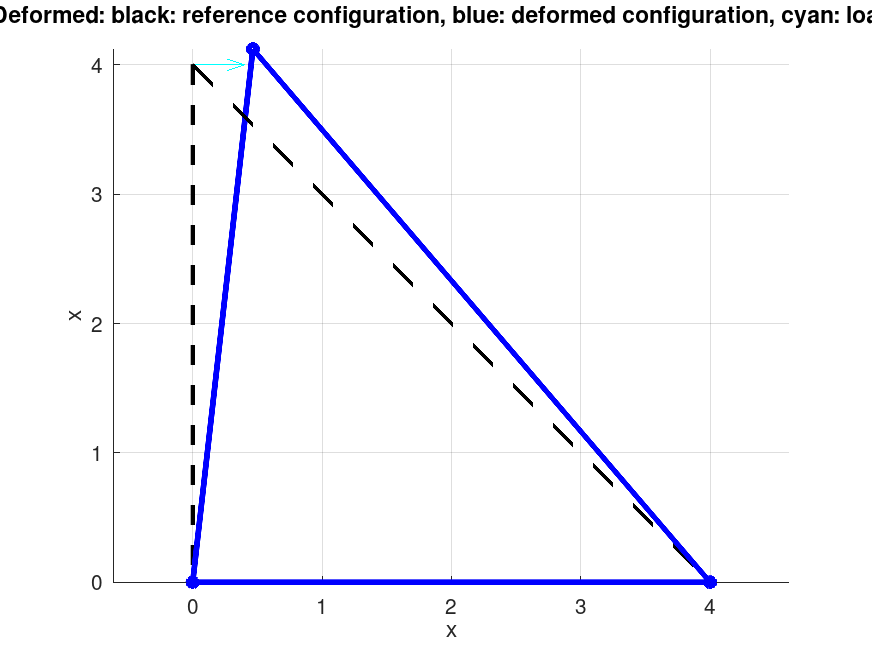
\includegraphics[width=0.65\textwidth]{deformed}
	\caption{Gráficos de deformada generado por el código FEMTrusS para el ejemplo presentado usando un factor de escala 1000.}
	\label{fig:ejbarraDef}
\end{figure}


En la Figura~\ref{fig:ejbarraDir} se muestra el diagrama de directas, también generado usando FEMTrusS.  %

\begin{figure}[htb!]
	\centering
	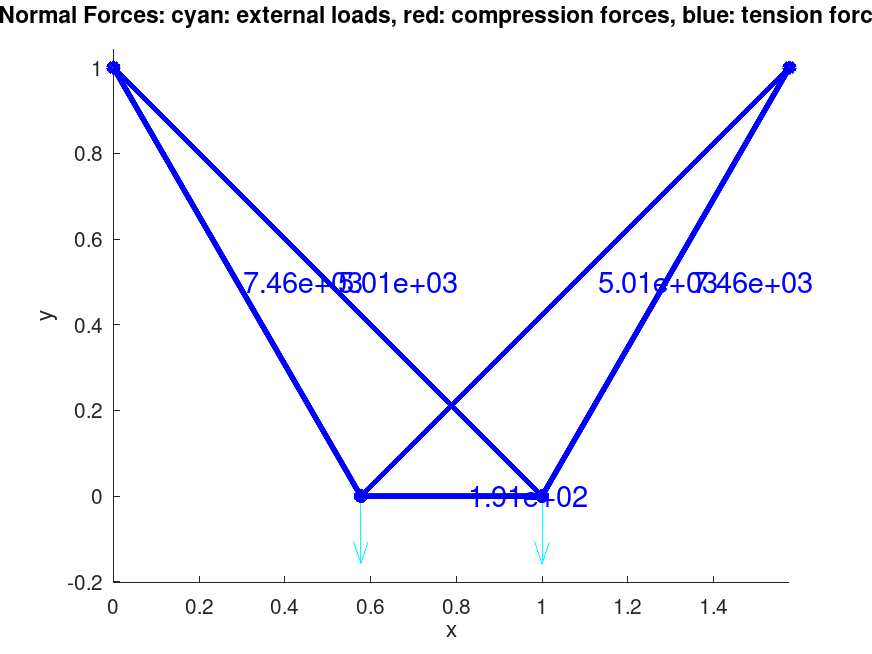
\includegraphics[width=0.65\textwidth]{normalforces}
	\caption{Gráficos de directas generado por el código FEMTrusS para el ejemplo presentado.}
	\label{fig:ejbarraDir}
\end{figure}



Finalmente, se menciona que si se considerara un resorte horizontal de constante elástica $k$ en el nodo 2 entonces se agregaría el término de energía potencial de deformación: $\frac{1}{2} k u_2^2$. %
%%
Luego de realizar las derivadas establecidas por Castigliano se obtendría $k u_2$, término que es considerado en el sistema lineal reducido como
%
\begin{equation}
\bfK =
\left[
\begin{matrix}
14.84 \times10^6 +k & 0 \\
0 & 224.84 \times10^6 
\end{matrix}
\right]
\end{equation}
%
lo cual resultaría en, como es esperado, un menor valor de desplazamiento nodal.




%%%%%%%%%%%%%%%%%%%%%%%%%%%%%%%%%%%%%%%%%%%%%%%%%%%%%%%%%%%%%%%%
%%%%%%%%%%%%%%%%%%%%%%%%%%%%%%%%%%%%%%%%%%%%%%%%%%%%%%%%%%%%%%%%
% metodo de las fuerzas
%%%%%%%%%%%%%%%%%%%%%%%%%%%%%%%%%%%%%%%%%%%%%%%%%%%%%%%%%%%%%%%%
%%%%%%%%%%%%%%%%%%%%%%%%%%%%%%%%%%%%%%%%%%%%%%%%%%%%%%%%%%%%%%%%
\section{Método de las Fuerzas}


El Método de las Fuerzas (MF) utiliza un enfoque de resolución complementario al MD. El MF considera las ecuaciones de equilibrio de fuerzas y tiene como objetivo primario determinar las incógnitas de fuerzas indeterminadas por esas ecuaciones. %
%
En el MD se utilizan principalmente ecuaciones constitutiva y de  compatibilidad cinemática, con el objetivo de obtener los desplazamientos.


En esta sección (y en el curso) se presenta el método orientado únicamente al análisis de reticulados, utilizando un enfoque similar al usado en \citep{Reddy2002b}. %
El MF puede ser aplicado al análisis de cualquier estructura hiperestática, los estudiantes interesados en la aplicación del MF a estructuras como pórticos pueden acudir a textos como \citep{Krenk2013,Fuchs2016} disponibles\footnote{Acceso variable año a año, definido por el financiamiento destinado a la ANII.} en la colección \textit{Springer} en \href{http://timbo.org.uy/}{timbo.org.uy}.
%


Tal como fue visto, los desplazamientos son la incógnita principal del MD. %
En el caso del MF los valores de las directas en las barras y las reacciones de los vínculos son la incógnita principal a determinar. %
%
Para ello se cuenta con las ecuaciones de equilibrio, condiciones de compatibilidad de desplazamientos y principios energéticos.


En el caso de estructuras isostáticas las ecuaciones de equilibrio permiten determinar el estado tensional y solicitaciones de la estructura de forma única, por lo que el MF no puede ser aplicado de forma directa. %
%
%
Nos enfocaremos en estructuras con grado de hiperestaticidad $gh$ positivo, para las cuales las directas $\textbf{N}$ y las reacciones $\textbf{R}$ que se encuentran en equilibrio con las fuerzas externas pueden ser calculadas como combinación de estados llamados canónicos. %

\cajaactividad{Enumerar las $9$ incógnitas de fuerzas (solicitaciones internas y reacciones) del Ejemplo de la Sección~\ref{sec:ejemplobarra}, aplicar las ecuaciones de equilibrio y despejar todas las incógnitas en función de la directa de la barra 3 ($N^3$). %
Escribir el conjunto de los vectores de $\bbR^9$ que cumplen el equilibrio como una suma de vectores dependientes de $P$ y $N^3$.}


\subsection{Estados Canónicos}

Los estados canónicos serán considerados como: estados tensionales que pueden ser combinados para obtener el estado tensional real de una estructura hiperestática. %
%
Estos estados canónicos pueden ser obtenidos liberando vínculos internos y/o externos de una estructura hiperestática original, hasta obtener una estructura isostática.

En la Figura~\ref{fig:estadoscanon} se muestra un ejemplo de una estructura hiperestática con $gh=2$, con un vínculo de hiperestaticidad interno y uno externo, por lo que se obtiene una estructura isostática ''cortando'' una barra y liberando un vínculo de uno de los apoyos. %


\begin{figure}[htb]
	\centering
	\def\svgwidth{0.95\textwidth}
\input{figs/UT2/MF.pdf_tex}
	\caption{Ejemplo de descomposición de estados canónicos para aplicación del MF.}
	\label{fig:estadoscanon}
\end{figure}

El estado fundamental $E_0$ corresponde a la estructura isostática resultante sometida a las fuerzas externas. %
%
El estado $E_1$ corresponde a la misma estructura isostática considerando dos fuerzas aplicadas en los extremos intermedios obtenidos luego del corte de la barra. Estas fuerzas unitarias consideradas corresponden a una directa unitaria en la barra cortada. %
%
En el estado $E_2$ se considera una fuerza horizontal correspondiente al vínculo liberado.
%
%Los valores de las fuerzas son multiplicados por un factor $X_1$.
% --------------------------------------



Se puede considerar que las fuerzas externas consideradas en la estructura son una combinación de las fuerzas externas correspondientes a cada estado canónico
%
\begin{equation}\label{eqn:fueX}
\bff(\bfX) = \bff_0 + \sum_{j=1}^{gh} X_j \bff_j,
\end{equation}
donde  $\bff_0$ representa el vector de fuerzas externas aplicadas a la estructura original, $\bff_j$ corresponde a las fuerzas de cada estado canónico y $\bfX$ es el vector de multiplicadores de cada estado.
%
En el ejemplo, $\bff_1$ corresponde a un vector con dos fuerzas unitarias colocadas en puntos muy cercanos dados por el corte de la barra (o bien en los nodos extremos de la barra cortada) y $\bff_2$ corresponde a un vector con la fuerza unitaria aplicada en el apoyo deslizante.

Por otra parte, las ecuaciones de equilibrio definen una relación entre directas y fuerzas externas. %
Esta relación entre directas de las barras y fuerzas externas aplicadas $N=N(\bff)$, donde las fuerzas externas de cada estado son conocidas. %
%
Usando la relación $\bff(\bfX))$ se puede obtener una expresión de directas considerando los factores $X_j$ como las incógnitas a determinar:
%
\begin{equation}\label{eqn:estadosdirectas}
\textbf{N}(\bfX) = \textbf{N}_0 + \sum_{j=1}^{gh} X_j \textbf{N}_j
\end{equation}
%
donde el subíndice $j$ representa los valores del estado $j$, $X_j$ representa un factor a determinar, $\bfN_0$ corresponde a las directas para el estado de cargas $\bff_0$ y $\bfN_j$ corresponde a las directas para el estado de cargas unitarias $\bff_j$.
%
% ------------


Esto mismo también es realizado para calcular las reacciones de la estructura:
%
\begin{equation}
\textbf{R}(\bfX) = \textbf{R}_0 + \sum_{j=1}^{gh} X_j \textbf{R}_j
\end{equation}

Si se considera que las directas $\bfN$ y las reacciones $\bfR$ son las incógnitas principales del método entonces, se puede decir que los estados canónicos permiten interpolar los posibles estados tensionales. Los estádos canónicos en el MF cumplen el rol de las funciones de interpolación de desplazamientos en el MD, mientras que los valores de las incógnitas $\bfX$ cumplen el rol de los desplazamientos nodales.

\subsection{Principios energéticos}

Hasta aquí se han presentado las fuerzas de los factores $X_j$ asociados a incógnitas de fuerza de los vínculos liberados del problema. %
%
Los valores de directas usados para calcular la energía de deformación complementaria, son obtenidos a partir de las relaciones directas-fuerzas externas del equilibrio de fuerzas. %
%
Se destaca que no se han tomado en consideración las condiciones cinemáticas establecidas por las condiciones de apoyo de la estructura, el principio de mínima energía potencial complementaria permite obtener condiciones para esto.


Para presentar el método de las fuerzas se deben introducir los conceptos de energía de potencial complementaria. %

\subsubsection{Energía potencial de deformación complementaria}
%
La energía potencial de deformación presentada $\Pi_{int}$ puede ser escrita en términos de las tensiones en lugar de los desplazamientos. %
%
Consideremos la energía de deformación de un elemento de barra:
%
\begin{equation}
\Pi_{int}^e(\bfu^e) = \frac{1}{2} \int_0^{\ell^e} \varep^e(\bfu^e) E^e A^e \varep^e(\bfu^e) dx
\end{equation}
%
usando la ecuación constitutiva se obtiene una expresión en función de la tensión del elemento
%
\begin{equation}
\Pi_{int}^e(\bfu^e) = \frac{1}{2} \int_0^{\ell^e} \sigma^e \sigma^e \frac{1}{E^e} A^e dx = (\Pi_{int}^*)^e(\sigma^e) 
\end{equation}
%
donde $\Pi_{int}^*$ representa la energía de deformación complementaria de la barra. %
%
En el caso de materiales elástico-lineales, como los considerados en este documento, la energía complementaria $\Pi_{int}^*$ coincide con la energía de deformación $\Pi_{int}$.
% ----------------------------

Usando que no hay fuerzas de volumen aplicadas a la barra y considerando la directa de la barra $N^e = \sigma^e A^e$ se obtiene una expresión de la energía en función de la directa:
%
\begin{equation}
(\Pi_{int}^*)^e(\bff) = \frac{1}{2} \frac{(N^e (\bff))^2}{E^e A^e} \ell^e.
\end{equation}
%
donde las fuerzas externas $\bff$ están relacionadas con la directas a través de las ecuaciones de equilibrio. %
%
La energía de deformación complementaria de la estructura completa está dada por la suma:
%
\begin{equation}\label{eqn:Udef}
\Pi_{int}^*(\bff) =  \frac{1}{2} \sum_{e=1}^{n_e} \frac{(N^e (\bff))^2}{E^e A^e} \ell^e.
\end{equation}

Para estructuras hiperestáticas, se puede considerar la relación entre $\bff$ y $\bfX$ y considerar el vector $\bfX$ como variable:
%
\begin{equation}
\boxed{
(\Pi_{int}^*)^e(\bfX) = \frac{1}{2} \frac{(N^e (\bfX))^2}{E^e A^e} \ell^e.
}
\end{equation}

\subsubsection{Energía potencial complementaria de cargas externas}
La energía potencial de las cargas externas $\Pi_{ext}$ puede ser considerada también como una función de las fuerzas externas aplicadas, de la forma:
%
\begin{equation}\label{eqn:Vdef}
\Pi_{ext}(\bfu) = -\bfu^T \bff = \Pi_{ext}^*(\bff).
\end{equation}





\subsubsection{Energía potencial complementaria total}

La energía potencial complementaria total puede también ser escrita en función de las variables $\bfX$. %
%
Sustituyendo la Ecuación~\eqref{eqn:estadosdirectas} en la definición de $\Pi_{int}^*$ (Ecuación~\eqref{eqn:Udef})  y la Ecuación~\eqref{eqn:fueX} en la definición de $\Pi_{ext}^*$ (Ecuación~\eqref{eqn:Vdef}) se obtiene:
%
\begin{equation}
\Pi^* (\bfX) = \frac{1}{2}  \sum_{e=1}^{n_e} \frac{(N_0^e + \sum_{j=1}^{gh} X_j N_j^e)^2}{E^e A^e} \ell^e - \bfu^T \bff_0 - \bfu^T \left( \sum_{j=1}^{gh} X_j \bff_j \right).
\end{equation}


\subsubsection{Mínima energía potencial complementaria total}

El principio de mínima energía potencial complementaria total establece que dada una estructura con ciertas condiciones de apoyos y un conjunto de fuerzas externas aplicadas, la distribución de fuerzas internas en equilibrio compatible con los vínculos de los desplazamientos es aquella que minimiza la energía potencial complementaria total de la estructura. Esto puede ser escrito en función de los factores $X_j$, de la forma:
%
\begin{equation}
\textbf{X} = \argmin_{\textbf{X} \in \bbR^{gh} } \Pi^*(\textbf{X}).
\end{equation}

\subsubsection{Segundo teorema de Castigliano}

El segundo Teorema de Castigliano consiste básicamente en las condiciones de optimalidad del problema de mínimo de energía potencial complementaria total, %
%
las cuales consisten en plantear gradiente nulo:
%
\begin{equation}
\frac{\partial \Pi^*}{ \partial X_i}(\bfX) = 0  \quad i=1,\dots,gh \Rightarrow 
\frac{\partial \Pi_{int}^*}{ \partial X_i}(\bfX) = \bfu^T \bff_i \quad i=1,\dots,gh.
\end{equation}
%
Considerando que los valores de fuerzas externas de los estados canónicos distintos al fundamental son unitarios se tiene:
%
\begin{equation}
\frac{\partial \Pi_{int}^*}{ \partial X_i}(\bfX) =  \delta_i \qquad i=1,\dots,gh
\end{equation}
%
donde $\delta_i$ representa el desplazamiento nodal (o la suma de varios desplazamientos) de la estructura como resultado de las cargas externas aplicadas en los puntos donde hay fuerzas unitarias aplicadas en el estado canónico $i$. %
%
Este desplazamiento deberá tomar un valor compatible con el vínculo que fue liberado. %

En los casos en los que el vínculo liberado está asociado a un desplazamiento nulo (continuidad o apoyos fijos) se tiene
%
\begin{equation}
\frac{\partial \Pi_{int}^*}{ \partial X_i}(\bfX) = 0 \qquad i=1,\dots,gh.
\end{equation}

En el ejemplo mostrado en la Figura~\ref{fig:estadoscanon}, para el estado 1 el desplazamiento corresponde a la resta de los desplazamientos de los nodos obtenidos luego del corte, lo cual, dado que hay continuidad, debe ser cero. %
%
Para el estado 2 el desplazamiento corresponde a cero ya que el vínculo liberado corresponde a un apoyo fijo. %
%


\subsection{Método de las Fuerzas para análisis de reticulados}

En esta sección se presentan esquemáticamente las ecuaciones del MF para el análisis de reticulados.


El método consiste en liberar $gh$ vínculos de la estructura para obtener una estructura isostática y aplicar las ecuaciones del segundo teorema de Castigliano, imponiendo el desplazamiento correspondiente a los vínculos liberados. %

En el caso de estructuras de barras articuladas donde los vínculos liberados tienen desplazamiento nulo, y aplicando el segundo teorema de Castigliano se tiene:
%
\begin{equation}
 \frac{\partial \Pi_{int}^*}{ \partial X_i}(\bfX) =  \sum_{e=1}^{n_e} \frac{N_i^e(N_0^e + \sum_{j=1}^{gh} X_j N_j^e)}{E^e A^e} \ell^e = 0
 \qquad i=1,\dots, gh
\end{equation}
%
donde se consideró que el desplazamiento de cada estado corresponde a un valor nulo. %

Desarrollando el producto se obtienen $gh$ condiciones
\begin{equation}
\sum_{j=1}^{gh}  X_j \left( \sum_{e=1}^{n_e}  \frac{ N_j^e N_i^e } {E^e A^e} \ell^e \right) = - \sum_{e=1}^{n_e} \frac{N_i^e N_0^e } {E^e A^e} \ell^e \qquad i=1,\dots,gh,
\end{equation}
%
lo que representa un sistema lineal de ecuaciones de $gh$ incógnitas y ecuaciones.
% ---------------------------


Escrito en forma matricial esto es:
\begin{equation}\label{eqn:ecflex}
\bfM_f \bfX = \bfb_f
\end{equation}
%
donde $\bfM_f$ es llamada matriz de flexibilidad y sus entradas están dadas por:
%
\begin{equation}
(\bfM_f)_{ij} =  \sum_{e=1}^{n_e} \frac{N_i^e N_j^e }{E^e A^e} \ell^e,
\end{equation}
y el término independiente $\bfb_f$ está dado por:
%
\begin{equation}
(\bfb_f)_{i} =  - \sum_{e=1}^{n_e} \frac{N_0^e N_i^e }{E^e A^e} \ell^e.
\end{equation}

La Ecuación~\eqref{eqn:ecflex} es llamada ecuación de flexibilidad.
	
\subsubsection{Procedimiento práctico de aplicación}

\begin{enumerate}
\item calcular el grado de hiperestaticidad de la estructura $gh$,
\item si $gh$ es positivo entonces liberar $gh$ vínculos de la estructura obteniendo $gh+1$ esquemas básicos de estructuras isostáticas (estados canónicos),
\item calcular las directas y reacciones para cada uno de los estados canónicos,
\item calcular la matriz de flexibilidad y el término independiente,
\item calcular los factores de cada estado $X_j$ resolviendo la ecuación de flexibilidad,
\item calcular los valores de directa y reacciones solución sustituyendo los valores $X_j$.
\end{enumerate}


\subsubsection{Cálculo de desplazamiento}

El segundo teorema de Castigliano puede ser aplicado también para calcular el desplazamiento de cualquier punto de la estructura. %
%
Dado un vector de fuerza $\bfX_{sol}$ obtenido como solución de la ecuación de flexibilidad, se considera un estado canónico adicional $E_{gh+1}$ con una fuerza externa unitaria según el desplazamiento deseado. %
%
Se aplica Castigliano y a través de la derivada de la energía respecto el valor correspondiente de $X$ y considerando que este valor $X$ debe ser nulo se obtiene el desplazamiento deseado. %
%
\begin{equation}
\delta_{gh+1} = \frac{\partial \Pi^*_{int}}  { \partial X_{gh+1} } (\bfX = \bfX_{sol}, X_{gh+1}=0)
\end{equation}

Existe un caso particular destacable. %
%
Si en el estado canónico $E_0$ existe una única fuerza aplicada de magnitud $P$, y además el estado canónico $E_{gh+1}$, necesario para calcular el desplazamiento, cumple que $E_0 = P E_{gh+1}$, entonces se puede probar que %
%
\begin{equation}
\delta_{gh+1} = \frac{\partial \Pi^*_{int}}  { \partial P } (\bfX = \bfX_{sol}, X_{gh+1}=0).
\end{equation}
%



\subsection{Implementación computacional}

La implementación computacional del procedimiento del Método de las Fuerzas no es tan directa como la del Método de los Desplazamientos. %
%
A pesar de esto, se brinda un ejemplo de implementación, que puede ser también estudiado por los estudiantes interesados en entender el procedimiento planteado por el método. %

Los códigos están disponibles en el repositorio \href{https://github.com/jorgepz/FDMTrusS}{github.com/jorgepz/FDMTrusS}, y se aclara que el código es una versión minimal, en proceso de revisión, que aspira simplemente a mostrar una posible forma de automatizar el proceso del Método y  \textbf{no forma parte de los contenidos} centrales \textbf{del curso} y no será evaluado directamente. %
%



\subsection{Ejemplo de Método de las Fuerzas}

Se presenta la resolución del mismo problema de la Sección~\ref{sec:ejemplobarra}, en este caso usando el MF. %
%
Se comienza calculando el grado de hiperestaticidad como $gh= 3 + 6 - 2 \times 4 = 1$.


En este problema existen más de una posibilidad de estados canónicos a considerar. En la Figura~\ref{fig:hipereje} se muestran los estados canónicos elegidos, considerando un corte en la barra 2-4.

\begin{figure}[htb]
\centering
\def\svgwidth{\textwidth}
\input{figs/UT2/Ej_UT2_retic_MF.pdf_tex}
\caption{Estados canónicos de ejemplo.}
\label{fig:hipereje}
\end{figure}

Las directas en las barras para cada uno de los estados están dadas por la siguiente tabla.
	\begin{center}
		\begin{tabular}{cccc}
\hline
			Elemento & $N_0$ &  $N_1$ & $ \ell / E A$ \\
			\hline
			1 & $\sqrt{2} P$ & 1 & $6.73 \times 10^{-8}$ \\
			2 & -$P$ & -$\sqrt{2}$ & $4.76 \times 10^{-9}$ \\
			3 & 0 &  1 & $ 6.73 \times 10^{-8}$ \\
			\hline
		\end{tabular}
	\end{center}

Usando las ecuaciones del segundo teorema de Castigliano  se obtiene:
%
\begin{equation}
X_1 \cdot  1.44 \times 10^{-7} = -1.02 \times 10^{-3} \Rightarrow \boxed{ X_1 = -7071 \, \text{N} }.
\end{equation}

Las directas en las barras son calculadas usando la ecuación Ecuación~\eqref{eqn:estadosdirectas}:
%
\begin{equation}
N^1 = - N^3 =7.07 \, \text{kN} \quad \text{y} \quad N^2 = 0.
\end{equation}
obteniendo un resultado que coincide con el obtenido usando el MD.



Para determinar los desplazamientos usando el teorema de Castigliano es posible considerar un estado canónico adicional auxiliar con una fuerza aplicada según la dirección y sentido del desplazamiento deseado. %
%
Este estado adicional agrega una fuerza que no existe en la estructura y que por lo tanto debe ser nula. Se calcula la energía de deformación correspondiente a todos los estados, se calcula la derivada y en ese momento se impone que el valor de el factor correspondiente a este estado es cero.

A modo de ejemplo se determinará el desplazamiento horizontal del nodo 2 en el ejemplo. %
%
Para esto se considera un estado $E_2$ vinculado a una fuerza unitaria hacia la derecha aplicada en el nodo 2 multiplicada por un factor $X_2$. %
%
En este estado las directas son $N_2^1 = \sqrt{2}, N_2^2 = -1, N_2^3 = 0$.


La energía de deformación complementaria está dada por
%
\begin{equation}
\Pi_{int}^*(\bfX) = \frac{1}{2}  \sum_{e=1}^{n_e} \frac{(N_0^e +   \sum_{j=1}^{gh+1}  X_j N_j^e)^2}{E^e A^e} \ell^e 
\end{equation}

Calculando la derivada y evaluando en $X_2=0$ (debido a que la fuerza agregada debe ser nula) y $X_1$ igual al valor obtenido anteriormente, se obtiene:
\begin{equation}
\frac{\partial \Pi_{int}^*}{\partial X_2} (X_1=-7071,X_2=0) =  \sum_{e=1}^{n_e} \frac{N_2 (N_0^e +  X_1 N_1^e + 0 \, N_2^e  )}{E^e A^e} \ell^e  = 6.74 \times 10^{-4} \, \text{m}
\end{equation}
resultado que también coincide con el obtenido usando el MD.


En el caso de desear determinar otro desplazamiento se debe considerar un estado de fuerzas correspondiente siempre considerados sobre la estructura ísostática fundamental.


\newpage
\section{Ejercicios}
\setcounter{ejercicio}{0}

\ejercicio


Considere el reticulado de la figura donde todas las barras están construidas con barras de acero ($E=210$ GPa) de sección tubular con $\phi_{ext} =100$ mm y espesor $t=5$ mm. 

\begin{center}
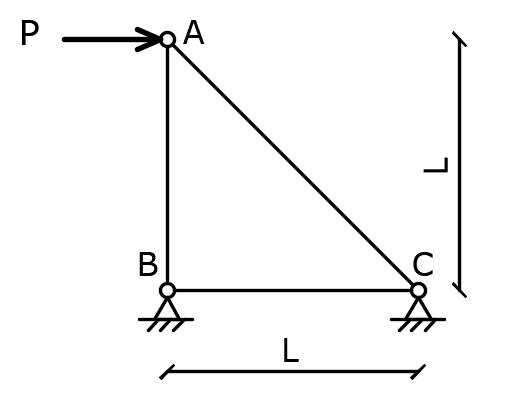
\includegraphics[width=0.45\linewidth]{UT2ej1}
\end{center}

Considerando que $P=50$ kN y $L=4.0$ m, se pide:

\parte Calcular las reacciones, los esfuerzos en todas las barras y el desplazamiento del nodo A mediante el Método de los Desplazamientos y el Método de las Fuerzas.

\parte Verificar lo hallado en la parte anterior mediante el empleo de alguna herramienta computacional.




\ejercicio

En la estructura reticulada mostrada en la figura cada barra está formada por 2 perfiles PNC10 de acero ($E=210$ GPa).

\begin{center}
	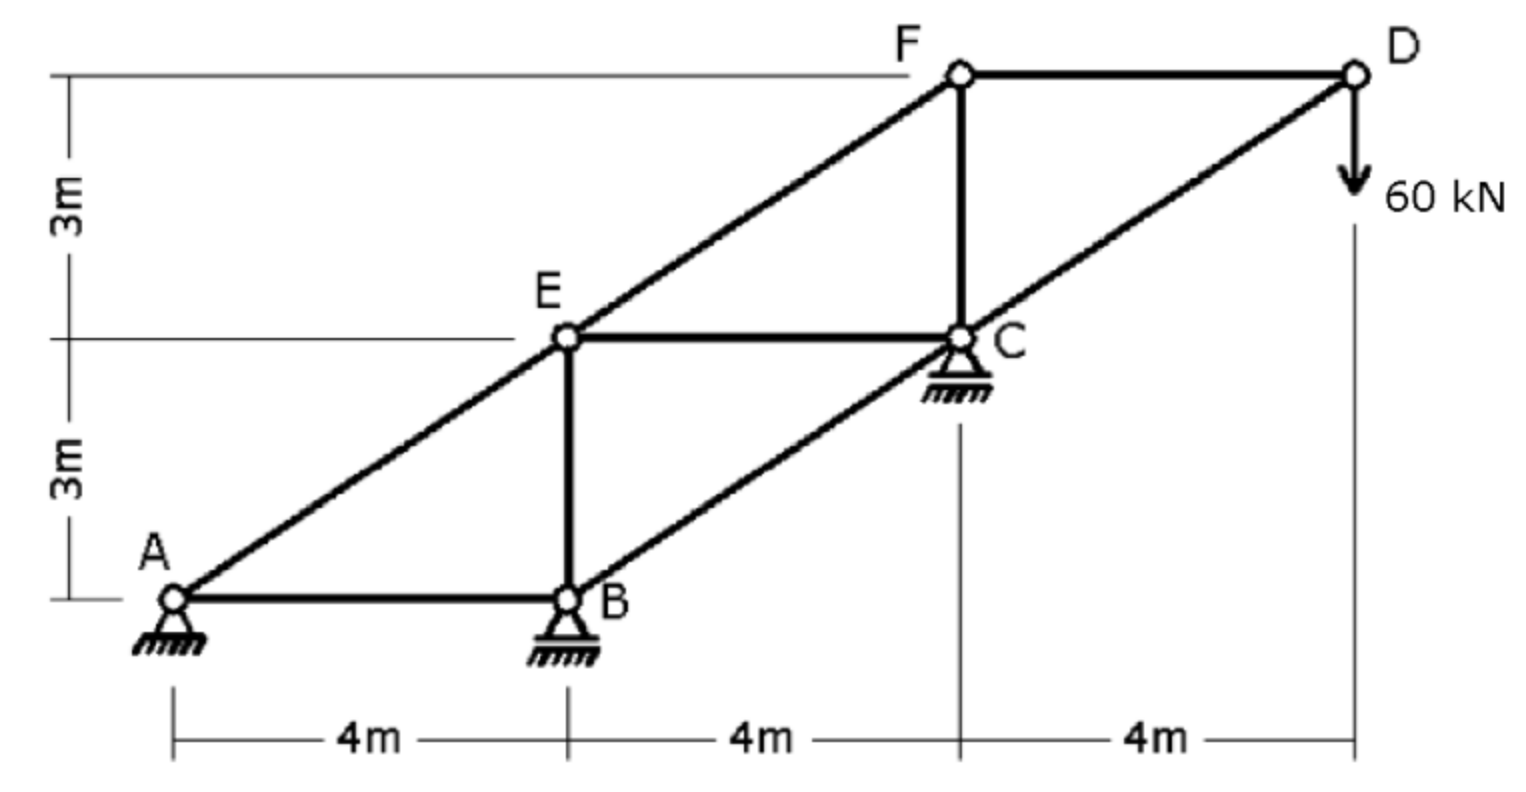
\includegraphics[width=0.8\linewidth]{UT2ej2}
\end{center}

Se pide:
%
\parte Calcular las reacciones, los esfuerzos en todas las barras y el desplazamiento del nodo D mediante el método de las fuerzas.
%
\parte Verificar lo hallado en la parte a) mediante el empleo de alguna herramienta computacional.




\ejercicio

En la estructura reticulada mostrada en la figura todas las barras tienen la misma sección y están formadas por el mismo material. %

\begin{center}
	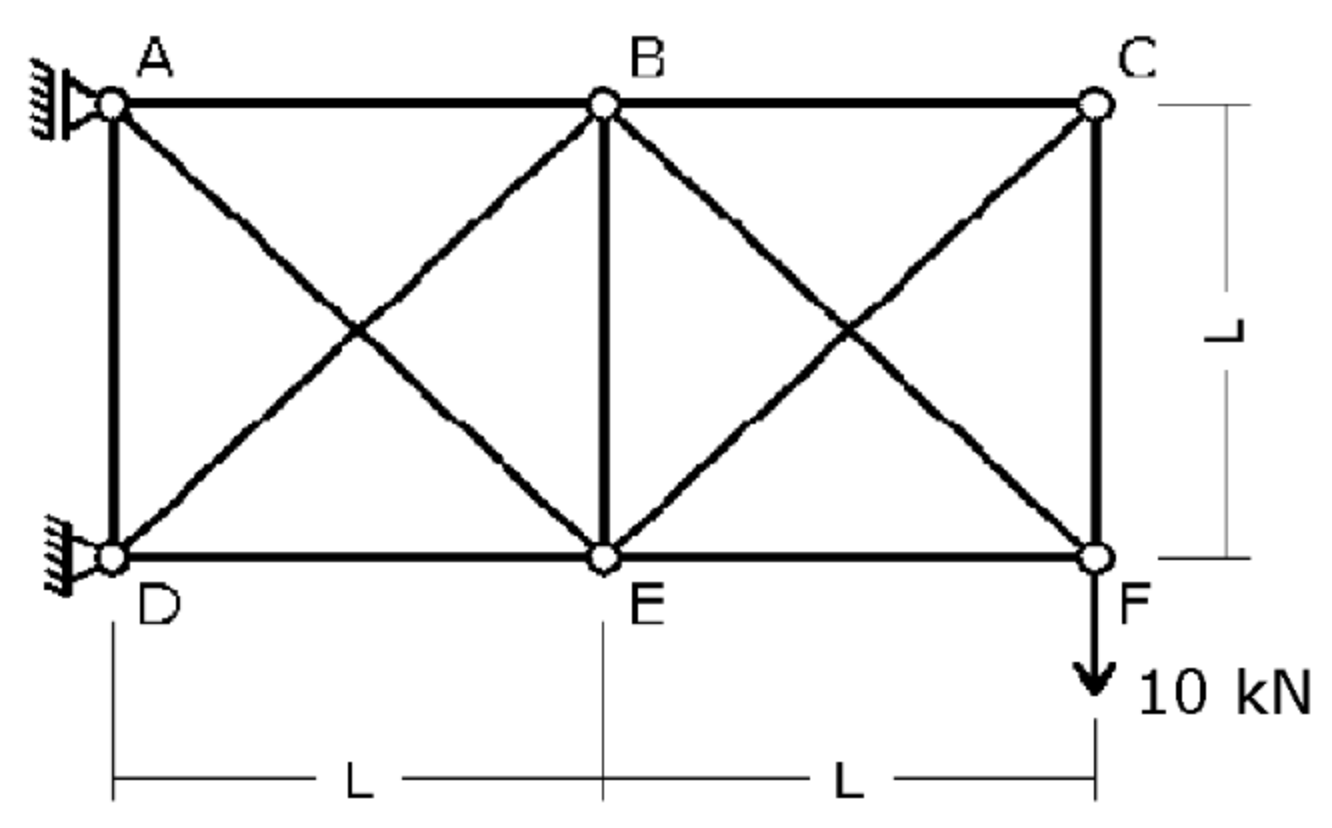
\includegraphics[width=0.6\linewidth]{UT2ej3}
\end{center}

Aplicando el Método de las Fuerzas, se pide:

\parte Calcular las reacciones y los esfuerzos en todas las barras.
%
\parte Si $L=1$ m, el área de cada barra $\Omega=4$ cm$^2$ y $E=210$ GPa, calcular el desplazamiento del nodo F.
%
\parte Verificar lo hallado en la parte a) y b) mediante alguna herramienta computacional.


\ejercicio

En la estructura reticulada mostrada en la figura, todas las barras tienen la misma sección y el mismo material.

\begin{center}
	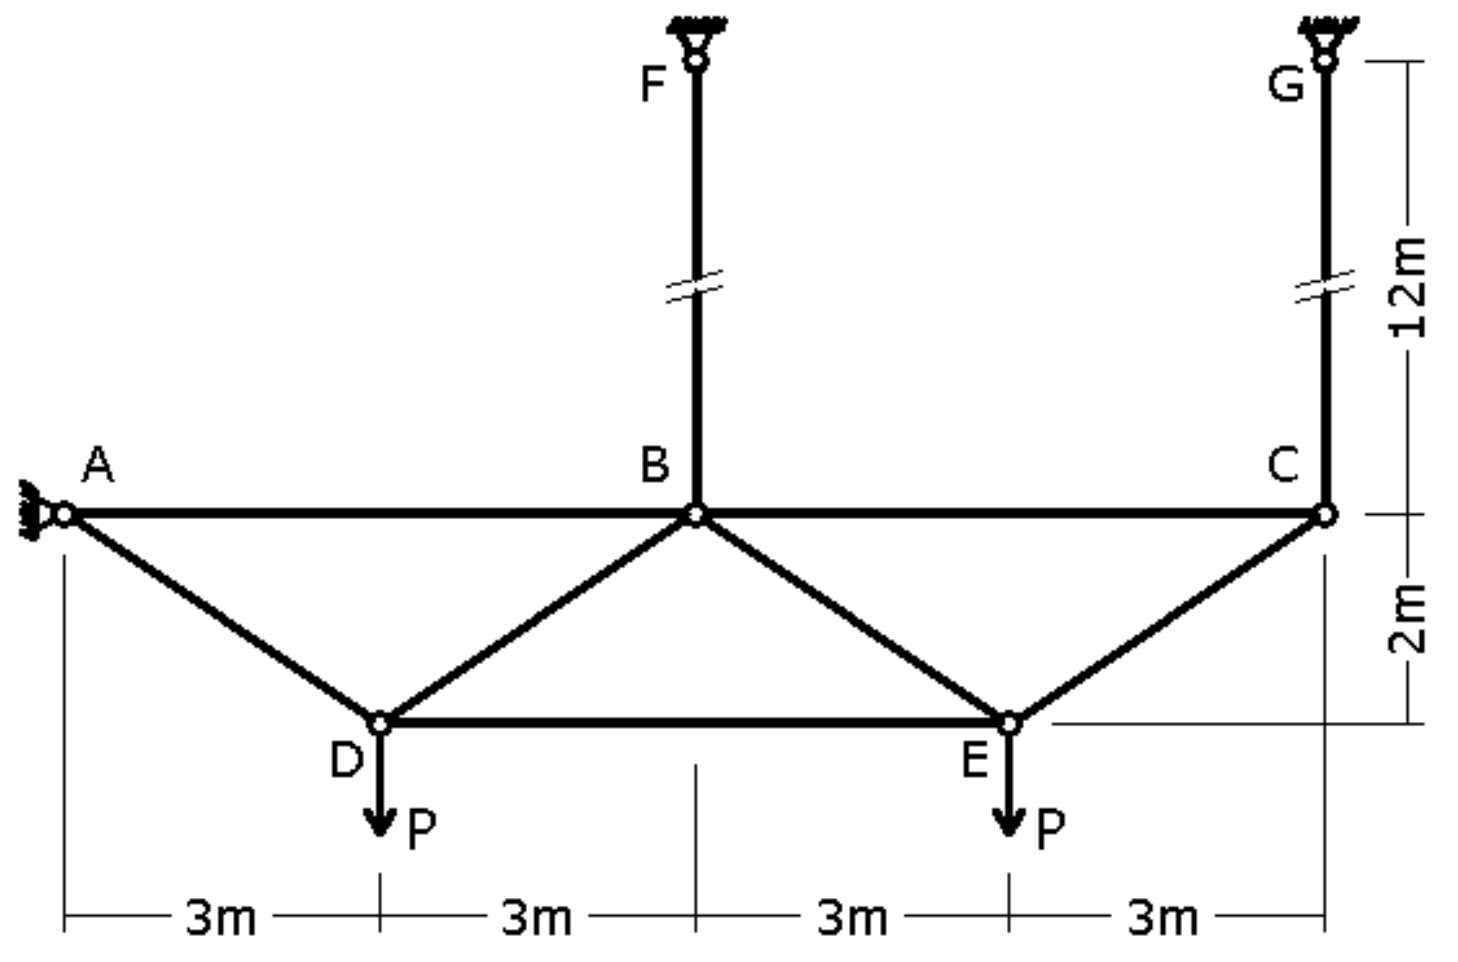
\includegraphics[width=0.75\linewidth]{UT2ej4}
\end{center}

Considerando  $P=10$ kN, $E=210$ GPa y $\Omega=1$ cm$^2$, se pide:
%
\parte Mediante el método de las fuerzas calcular las reacciones, los esfuerzos en todas las barras y el desplazamiento vertical de los nodos B y C. 
%
\parte Verificar lo hallado en la parte a) mediante alguna herramienta computacional.


\ejercicio
Sea el reticulado y las cargas que se muestran en la figura, donde todos los triángulos son equiláteros y las barras tienen todas mismo módulo de elasticidad y área.

\begin{center}
	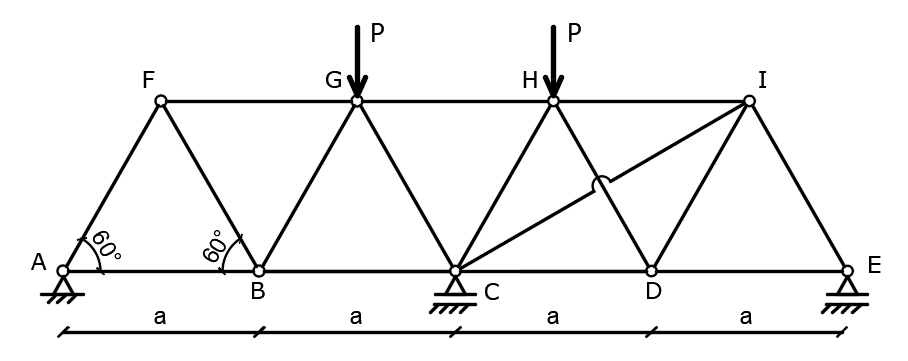
\includegraphics[width=0.95\linewidth]{UT2ej5}
\end{center}

Se pide:

\parte Calcular la solicitación de cada barra utilizando el método de las fuerzas.
\parte Dimensionar la estructura con perfiles PNI, suponiendo que todas las barras son iguales, para $P=300$ kN, $a=3$ m y $\sigma_{adm}=140$ MPa.

